\documentclass[a4paper, 11pt]{article}

\usepackage[utf8]{inputenc}

\usepackage[T1]{fontenc}

\usepackage[english]{babel}

\usepackage{graphicx}

\usepackage{multicol}

\usepackage{floatrow}

\usepackage[margin = 1in]{geometry}

\usepackage{float}

\usepackage[hidelinks, urlcolor=cyan]{hyperref}

\usepackage{url}

\usepackage{natbib}

\bibliographystyle{abbrvnat}
\setcitestyle{authoryear,open={(},close={)}}

\usepackage{csquotes}

\usepackage{fancyhdr}

\usepackage{lipsum}

\usepackage{adjustbox}
\usepackage{rotating}
\usepackage[table,xcdraw]{xcolor}

%\addbibresource{references.bib}

\title{\Large BINF-F401 Project \\
\huge Title}


\author{
	Draguet Simon
	\and
	Godin Maximilien
	\and
	Guyot Léopold
	}

\date{\today}

\begin{document}

\pagestyle{fancy}
\setlength{\headheight}{32.3pt}
\fancyhead{}\fancyfoot{}
\fancyhead[L]{
\includegraphics[scale = 0.05]{figures/LOGO_Universite _libre_bruxelles.png}}
\fancyhead[R]{Title}
\fancyfoot[R]{\thepage}

\maketitle

\begin{multicols}{2}

\section{Introduction}
R \citep{R:2024}

\section{exploration of  clinical variables}
Description des variables .....  

\subsection{Distribution of the variables }

\begin{scriptsize}	
	
	\textbf{Associated script : \href{https://github.com/leopoldguyot/BINF-F401-Project/*}{.R}}
\end{scriptsize}

By examining the clinical variables through histograms, we can visualize their distribution. Most of the continuous variables do not seem to follow a normal distribution. For instance, the variable AGE appears to be asymmetric, exhibiting a right skew (fig X).
To now if the continuous variable were normally distributed, we used a Shapiro-Wilk test. The results showed that AGE, HGHT, BMI, TRISCHD all had p-value under 5\%, leading us to reject the null hypothesis, which say that the sample is drawn form a normally distributed population. However, for WGHT, it was higher than 5 , so we didn’t reject the null hypothesis (table X ) . 

To do further analysis, we need them to be normally distributed. We tried to apply various transformations like log, square root, square. Only the square transformation successfully normalized the AGE sample. 
Because we needed it to work on all the continuous variable, we finally chose to use the rank-based inverse normal transformation (INT). that first convert the variable into ranks, then map it to a normal distribution. 

$ Y^t_{i}=  \Phi^{-1}(r-C/N-2C+1) $

where $r_i$ is the ordinary rank of the $_ith$ case among the N observations and $\Phi^{-1}$ denotes the standard normal quantile (or probit) function.For the value of C we use C=3/8 \citep{beasley2009rank}.

If we look at the discrete variable, we can see that we don't have a balanced distribution. For example, for the variable AGE, there are more than twice as many males as females (fig x). For DTHHRDY, we can observe that most of the deaths occurred in ventilator cases (fig x). When conducting analysis, it's essential to keep these observations in mind as they can significantly influence the interpretation. 

\subsection{Correlations between the clinical variables}

Principal Component Analysis (PCA) is a method of determining individual profiles and linear relationships between variables, based on correlation coefficients. The various graphs produced by a PCA, notably the correlation circle, are therefore a good way of illustrating the links between different quantitative variables, and getting a general idea of these links. Nevertheless, the data we are considering here are also partly qualitative. It is therefore preferable to turn to a Factor Analysis of Mixed Data, i.e. an analysis that applies a PCA to quantitative variables and a Multiple Correspondence Analysis to qualitative variables. The various dimensions defined by this method can be used to characterize all the variables. The FAMD() function in the FactoMineR package was used, with the argument allowing the creation of a series of graphs.

\begin{figure}[H]
	\centering
	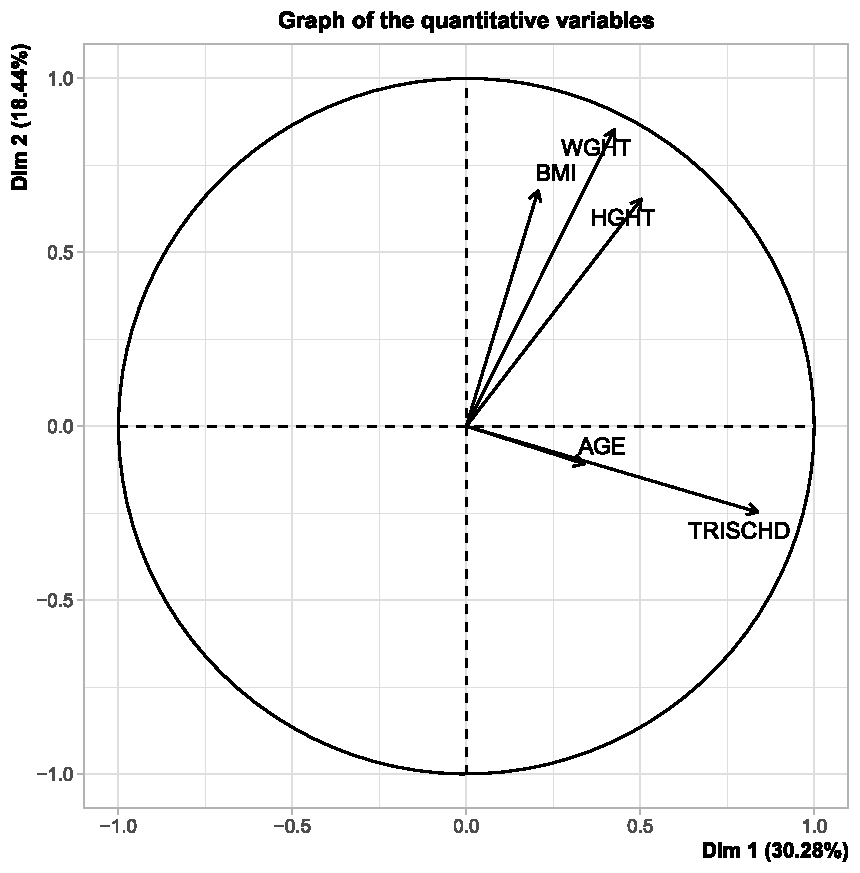
\includegraphics[width=\columnwidth]{figures/clinical_correlation_plots/all_quant_Dim2}
	\caption{Correlation circle of the continuous variables}
	\label{fig:corCircle}
\end{figure}

\begin{figure}[H]
	\centering
	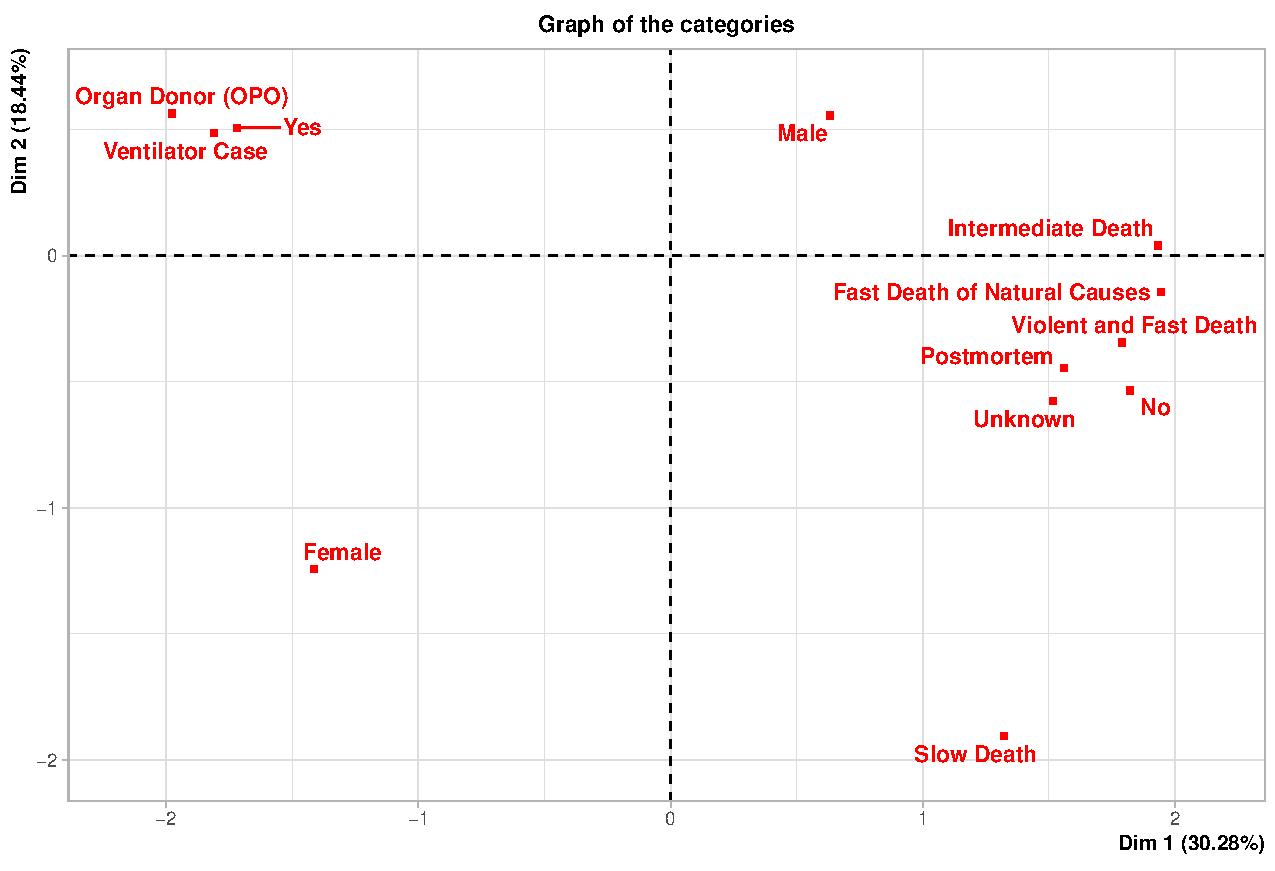
\includegraphics[width=\columnwidth]{figures/clinical_correlation_plots/all_categ_Dim}
	\caption{Level maps of all the different categories in the qualitative variables}
	\label{fig:lvlMap}
\end{figure}

The correlation circle allows us to represent quantitative variables according to the relationships they might have with each other, and the degree of explanation of these variables provided by the chosen dimensions. In this case, the two dimensions represented together explain only 48.72\% of the data, suggesting a certain complexity. 
This graph shows some correlation between the variables height (HGHT), weight (WGHT) and body mass index (BMI), which is not surprising given that taller people tend to be heavier, and also given that BMI is a function of height and weight. 
There also appears to be a correlation between age (AGE) and ischemic time (TRISCHD), i.e. the time between an individual's death and organ removal. This last observation is more difficult to explain intuitively. We can, however, point out that the variable AGE is weakly explained by the first two dimensions chosen, since its vector is close to the origin. This indicates that this possible correlation may not be significant, since by considering other dimensions, the vectors could be significantly far apart.

In contrast to the correlation circle, the level map represents the different categories or levels of categorical variables. We can already see that gender is close to different clusters. It would seem that there is a correlation between gender and type of death in these data, given that women seem to be more prone to ventilatory problems than men, which would explain the presence of a respirator before the person's death (Yes). It also appears that women are more likely than men to be organ donors. This graph therefore shows a certain correlation between gender and organ donation, type of death, but also between type of death and the presence or absence of a respiratory system prior to death.

Although these graphs illustrate the presence of possible correlations, they do not give any indication of their intensity, as they are not quantified. This quantification of correlation is particularly complex, as there is no correlation coefficient that can be applied to either quantitative or qualitative variables, or between these two types of variable. It was therefore decided to use different coefficients depending on the type of comparison, although this choice does not allow all correlations to be compared with each other. 
Correlations between quantitative variables were established using the cor() function with Spearman's method. This correlation was chosen because it does not require normally distributed variables, which is not the case for most of the variables considered. This coefficient is the only one to consider negative correlations.
Cramer's V was used to determine correlations between categorical variables, a coefficient based on the Chi-square statistic, and which is non-parametric. This correlation was calculated using the cramerV() function in the rcompanion package, with a bias correction given that this test tends to overestimate the relationships between categorical variables.
Logistic regression is used to determine the correlation between a quantitative variable and a binomial categorical variable, in this case gender and cohort. Finally, Cramer's V is applied to the H statistic of the Kruskall-Willis test between categorical and quantitative variables, as this statistic is the Kruskall-Willis chi-square. This application simply involves calculating the square root of the H statistic divided by the number of observations, the H statistic coming from the kruskall.willis() function.

\begin{figure}[H]
	\centering
	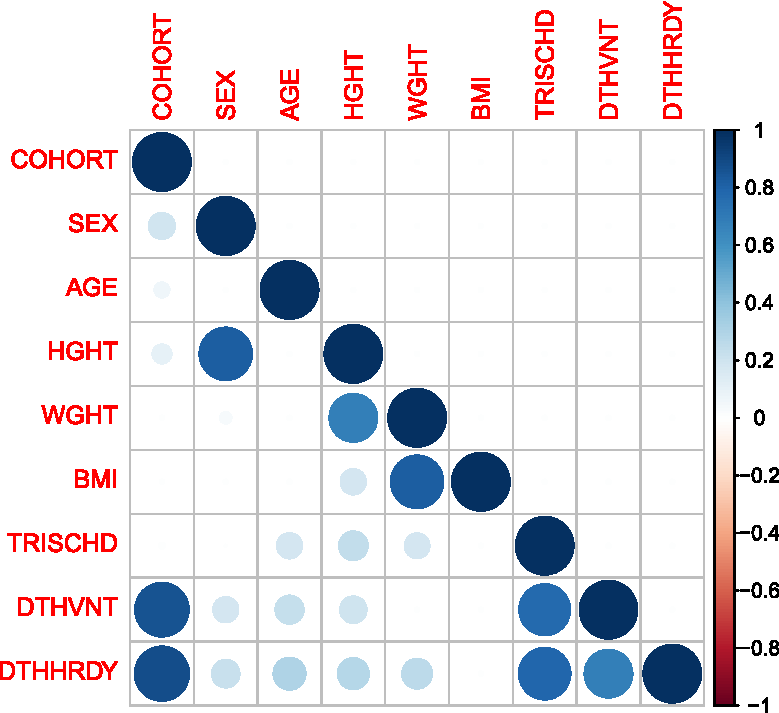
\includegraphics[width=\columnwidth]{figures/clinical_correlation_plots/corrected_allCorrelations2}
	\caption{Correlation matrix of all the variables}
	\label{fig:allCor}
\end{figure}

Looking at all the results together, we can see that there is a significant correlation between gender and height, which can simply be explained by the fact that men are generally taller than women. The correlation between height and weight, as well as between weight and BMI, can be explained as described above. Nevertheless, the absence of any significant correlation between height and BMI is rather odd given that the BMI calculation takes into account both height and weight, and that the correlation circle has positioned the corresponding vectors relatively close to each other. There is also a correlation between cohort and both type of death (DTHHRDY) and use of artificial ventilation before death (DTHVNT). There is a certain logic behind these correlations: the cohort variable divides people into organ donors and postmortem donors, i.e. victims of brain or cardiac death, thus depending on the type of death, but we can also consider that people with brain death are generally assisted with artificial ventilation before death. There also seems to be a correlation between the time between the individual's death and the removal of his or her organs and the type of death, but also the presence of a ventilatory apparatus. Finally, DTHVNT and DTHHRDY are also correlated.

\begin{table*}[t]
\footnotesize
\makebox[\linewidth]{
\begin{tabular}{|c|c c|c|c c|c c|c c|c|c c|c|cc|}
\cline{2-8}
    \hline & \multicolumn{2}{c|}{\rotatebox{90}{AGE}} & \rotatebox{90}{SEX} & \multicolumn{2}{c|}{\rotatebox{90}{HGHT}} & \multicolumn{2}{c|}{\rotatebox{90}{WGHT}} & \multicolumn{2}{c|}{\rotatebox{90}{BMI}} & \rotatebox{90}{COHORT} & \multicolumn{2}{c|}{\rotatebox{90}{TRISCHD}} & \rotatebox{90}{DTHVNT} & \multicolumn{2}{c|}{\rotatebox{90}{DTHHRDY}} \\
    \hline 
\rotatebox{90}{Cluster} &
  \rotatebox{90}{Normalized} &
  \rotatebox{90}{Categorical (56+ vs -56)} &
  \rotatebox{90}{Female vs Male} &
  \rotatebox{90}{Normalized} &
  \rotatebox{90}{Categorical (71+ vs -71)} &
  \rotatebox{90}{Normalized} &
  \rotatebox{90}{Categorical (181+ vs -181)} &
  \rotatebox{90}{Normalized} &
  \rotatebox{90}{Categorical (28+ vs -28)} &
  \rotatebox{90}{PostMortem vs OrganDonor} &
  \rotatebox{90}{Normalized} &
  \rotatebox{90}{Categorical (50+ vs -50)} &
  \rotatebox{90}{Yes vs No} &
  \rotatebox{90}{Intermediate vs Slow} &
  \rotatebox{90}{Fast vs Slow} \\
  \hline
0 &  & \cellcolor[HTML]{FDFF89}1,22 & \cellcolor[HTML]{B4F5F2}-1,26 &  &  &  &  &  &  & \cellcolor[HTML]{FDFF89}1,98 &  & \cellcolor[HTML]{FDFF89}1,78 & \cellcolor[HTML]{B4F5F2}-1,49 & \cellcolor[HTML]{FDFF89}2,10 & \cellcolor[HTML]{FDFF89}2,00 \\
1 &  &  &  &  &  &  &  &  &  &  &  &  &  &  &  \\
2 &  & \cellcolor[HTML]{FDFF89}1,87 & \cellcolor[HTML]{B4F5F2}-1,99 &  &  &  & \cellcolor[HTML]{FDFF89}1,15 &  & \cellcolor[HTML]{FDFF89}1,70 & \cellcolor[HTML]{FDFF89}2,46 &  & \cellcolor[HTML]{FDFF89}2,36 & \cellcolor[HTML]{B4F5F2}-2,38 & \cellcolor[HTML]{FDFF89}1,71 & \cellcolor[HTML]{FFC702}2,85 \\
3 &  &  &  &  &  &  &  &  &  & \cellcolor[HTML]{FDFF89}1,24 &  &  &  &  &  \\
4 &  &  &  &  &  &  &  &  &  &  &  &  &  &  &  \\
5 &  &  &  &  &  &  &  &  &  & \cellcolor[HTML]{FDFF89}1,55 &  & \cellcolor[HTML]{FDFF89}1,19 & \cellcolor[HTML]{B4F5F2}-1,41 &  &  \\
6 &  &  & \cellcolor[HTML]{FDFF89}1,70 & \cellcolor[HTML]{B4F5F2}-1,02 & \cellcolor[HTML]{B4F5F2}-2,32 &  &  &  &  & \cellcolor[HTML]{6F94FF}-5,33 &  & \cellcolor[HTML]{6F94FF}-5,91 & \cellcolor[HTML]{F56B00}6,27 & \cellcolor[HTML]{6F94FF}-6,34 & \cellcolor[HTML]{6F94FF}-5,90 \\
7 &  &  &  &  &  &  &  &  &  & \cellcolor[HTML]{B4F5F2}-1,10 &  &  &  &  &  \\
8 &  &  & \cellcolor[HTML]{FDFF89}1,03 &  &  &  &  &  &  & \cellcolor[HTML]{B4F5F2}-2,31 &  & \cellcolor[HTML]{B4F5F2}-2,02 & \cellcolor[HTML]{FDFF89}2,17 & \cellcolor[HTML]{B4F5F2}-2,25 & \cellcolor[HTML]{B4F5F2}-2,02 \\
9 &  &  &  &  &  &  &  &  &  & \cellcolor[HTML]{FDFF89}1,17 &  &  &  &  &  \\
10 &  & \cellcolor[HTML]{B4F5F2}-1,53 & \cellcolor[HTML]{FDFF89}1,07 &  & \cellcolor[HTML]{4AD7FF}-2,69 &  & \cellcolor[HTML]{4AD7FF}-2,60 &  &  & \cellcolor[HTML]{6F94FF}-6,72 & \cellcolor[HTML]{B4F5F2}-1,12 & \cellcolor[HTML]{6F94FF}-6,90 & \cellcolor[HTML]{F56B00}7,35 & \cellcolor[HTML]{6F94FF}-6,41 & \cellcolor[HTML]{6F94FF}-7,12 \\
11 &  &  &  &  &  &  &  &  &  &  &  &  &  &  &  \\
12 &  &  &  &  &  &  &  &  &  & \cellcolor[HTML]{B4F5F2}-1,32 &  &  & \cellcolor[HTML]{FDFF89}1,03 &  &  \\
13 &  &  &  &  &  &  &  &  &  &  &  &  &  &  &  \\
14 &  &  &  &  &  &  &  &  &  & \cellcolor[HTML]{B4F5F2}-1,84 &  & \cellcolor[HTML]{B4F5F2}-1,72 & \cellcolor[HTML]{FDFF89}1,78 & \cellcolor[HTML]{B4F5F2}-1,62 & \cellcolor[HTML]{B4F5F2}-1,58 \\
15 &  &  &  &  &  &  &  &  &  & \cellcolor[HTML]{FDFF89}1,25 &  & \cellcolor[HTML]{FDFF89}1,04 & \cellcolor[HTML]{B4F5F2}-1,03 &  &  \\
16 &  &  &  &  &  &  &  &  &  & \cellcolor[HTML]{FDFF89}1,48 &  & \cellcolor[HTML]{FDFF89}1,19 & \cellcolor[HTML]{B4F5F2}-1,07 & \cellcolor[HTML]{FDFF89}1,41 &  \\
17 &  &  &  &  &  &  &  &  &  & \cellcolor[HTML]{B4F5F2}-1,42 &  &  &  &  & \cellcolor[HTML]{B4F5F2}-1,20 \\
18 &  &  &  &  &  & \cellcolor[HTML]{FFC702}4,40 &  & \cellcolor[HTML]{FFC702}3,12 &  &  & \cellcolor[HTML]{6F94FF}-5,25 &  &  &  &  \\
19 &  &  &  &  &  &  &  &  &  &  &  &  &  &  &  \\
20 &  &  & \cellcolor[HTML]{FDFF89}1,02 &  &  &  &  &  &  & \cellcolor[HTML]{B4F5F2}-2,38 &  & \cellcolor[HTML]{B4F5F2}-2,07 & \cellcolor[HTML]{FDFF89}2,44 & \cellcolor[HTML]{B4F5F2}-2,43 & \cellcolor[HTML]{B4F5F2}-2,26 \\
21 &  &  & \cellcolor[HTML]{B4F5F2}-1,09 &  &  &  &  &  &  & \cellcolor[HTML]{FDFF89}1,83 &  & \cellcolor[HTML]{FDFF89}1,60 & \cellcolor[HTML]{B4F5F2}-1,69 & \cellcolor[HTML]{FDFF89}1,68 & \cellcolor[HTML]{FDFF89}1,73 \\
22 &  &  &  &  &  &  &  &  &  & \cellcolor[HTML]{FDFF89}1,47 &  & \cellcolor[HTML]{FDFF89}1,22 & \cellcolor[HTML]{B4F5F2}-1,26 & \cellcolor[HTML]{FDFF89}1,23 & \cellcolor[HTML]{FDFF89}1,02 \\
23 &  &  & \cellcolor[HTML]{FDFF89}1,28 &  & \cellcolor[HTML]{B4F5F2}-1,56 &  &  &  &  & \cellcolor[HTML]{4AD7FF}-4,53 &  & \cellcolor[HTML]{4AD7FF}-4,22 & \cellcolor[HTML]{F56B00}5,19 & \cellcolor[HTML]{6F94FF}-5,27 & \cellcolor[HTML]{4AD7FF}-4,91 \\
24 &  &  &  &  &  &  &  &  &  & \cellcolor[HTML]{FDFF89}2,19 &  & \cellcolor[HTML]{FDFF89}1,93 & \cellcolor[HTML]{B4F5F2}-1,61 & \cellcolor[HTML]{FDFF89}2,22 & \cellcolor[HTML]{FDFF89}2,09 \\
25 &  &  & \cellcolor[HTML]{FDFF89}1,59 &  & \cellcolor[HTML]{B4F5F2}-1,42 &  &  &  &  & \cellcolor[HTML]{6F94FF}-5,75 &  & \cellcolor[HTML]{6F94FF}-5,21 & \cellcolor[HTML]{F56B00}5,58 & \cellcolor[HTML]{6F94FF}-6,35 & \cellcolor[HTML]{6F94FF}-5,25 \\
26 &  &  &  &  &  &  &  &  &  & \cellcolor[HTML]{FDFF89}1,72 &  & \cellcolor[HTML]{FDFF89}1,17 & \cellcolor[HTML]{B4F5F2}-1,46 & \cellcolor[HTML]{FDFF89}1,28 & \cellcolor[HTML]{FDFF89}1,57 \\
27 &  &  &  &  & \cellcolor[HTML]{B4F5F2}-1,14 &  &  &  &  & \cellcolor[HTML]{4AD7FF}-3,09 &  & \cellcolor[HTML]{4AD7FF}-2,62 & \cellcolor[HTML]{FFC702}2,92 & \cellcolor[HTML]{4AD7FF}-3,27 & \cellcolor[HTML]{4AD7FF}-2,85 \\
28 &  &  &  &  &  &  &  &  &  &  &  &  &  &  &  \\
29 &  &  &  &  &  &  &  &  &  &  &  &  &  &  &  \\
30 &  &  &  &  &  &  &  &  &  &  &  &  &  &  &  \\
31 &  & \cellcolor[HTML]{B4F5F2}-1,57 &  &  & \cellcolor[HTML]{B4F5F2}-1,47 &  & \cellcolor[HTML]{B4F5F2}-1,72 &  & \cellcolor[HTML]{B4F5F2}-1,10 & \cellcolor[HTML]{4AD7FF}-4,27 & \cellcolor[HTML]{B4F5F2}-1,38 & \cellcolor[HTML]{4AD7FF}-4,64 & \cellcolor[HTML]{F56B00}5,01 & \cellcolor[HTML]{6F94FF}-5,77 & \cellcolor[HTML]{4AD7FF}-4,42 \\
\hline
\end{tabular}}
\caption{Significant fold changes for each variable considered in this project, we also considered to categorize the continous data as a possible way to have more significant results.}
\label{tab:Q2FC}
\end{table*}

\subsection{Impact of technical variables on clinical variables}

In this section, we investigate the influence of technical variables on clinical data and describe the methodology employed to isolate their effects.
To decouple the impact of technical variables from the data of interest, linear regression analyses were conducted.
Prior to regression, the data underwent transformation using inverse data normalization for numerical variables (cf. section 1.1).

From the preceding section where correlations between variables were examined, certain expectations were established.
Age was anticipated to be associated with TRISCHD, DTHHRDY, and COHORT, while height and weight were expected to be linked to the same variables.
Additionally, sex appeared correlated with DTHHRDY and COHORT. Surprisingly, BMI seemed uncorrelated with any technical variables.

For the technical variable DTHHRDY, a decision was made to group certain categories into three new categories: slow, intermediate, and fast.
This choice was made since more observations by categories would enhance statistical power.

Upon conducting linear regression (generalized linear regression in the case of the categorical variable sex), it was observed that age was dependent on cohort, sex was dependent on DTHHRDY, height was dependent on DTHHRDY, weight was dependent on DTHHRDY, and, surprisingly, BMI was dependent on both DTHHRDY and COHORT.

Subsequently, linear regression (or generalize d linear regression) was rerun for each variable of interest, utilizing only the significant technical variables from the overall models.
The residuals of these models were stored for further analysis.
These residuals represent the data of interest with the unwanted effects of the technical variables removed, providing a clearer understanding of the clinical data.

\bibliography{references}

\end{multicols}
\end{document}
